% This template was originally by R. Jacob Vogelstein
% Updated on March 1, 2010 by Noah J. Cowan


\documentclass[12pt,oneside,final]{thesis}

\usepackage[superscript]{cite}
\usepackage{amsmath,amsfonts}
\usepackage{graphicx}
\graphicspath{{./figs/}}
\usepackage{fixltx2e}
\usepackage{array}
% wrapfig is fragile: use sparingly
\usepackage{wrapfig} 
%\usepackage{times}  % Use this for ugly fonts

\usepackage{upgreek}
\usepackage{hyperref}
\usepackage{setspace}

\usepackage{booktabs}
\usepackage{multirow}
\usepackage{longtable}
\usepackage[font=singlespacing, labelfont=bf]{caption}
%\usepackage{CV}

\usepackage{enumitem}
\newlist{inlinelist}{enumerate*}{1}
\setlist*[inlinelist,1]{%
  label=(\arabic*),
}

\usepackage{fancyhdr}    % Use nice looking headers along with the required footer page numbers   
%\usepackage[hypertex]{hyperref}

%Define the header/footer style
\pagestyle{fancy}
\fancyhf{}
\setlength{\headheight}{15pt}
\lhead{\leftmark}
\cfoot{\thepage}
\renewcommand{\headrulewidth}{0pt}
\fancypagestyle{plain}{% Redefine ``plain'' style for chapter boundaries
\fancyhf{} % clear all header and footer fields
\fancyfoot[C]{\thepage} % except the center
\renewcommand{\headrulewidth}{0pt}
\renewcommand{\footrulewidth}{0pt}}

%\tolerance=10000

%\makeglossary % enable the glossary

\begin{document}

\title{Thesis Proposal : Modulo7 : A full stack Music Information Retrieval and Querying Engine based on music theory principles}
\author{Arunav Sanyal}
\degreemonth{May}
\degreeyear{2015} 
\thesis
\masterscience
\copyrightnotice


% add your chapters, best way is to have separate TeX files for each chapter
%% FRONTMATTER
\begin{frontmatter}

% generate title
\maketitle

\begin{abstract}

Music Information Retrieval (MIR) is an interdisciplinary science of extracting non trivial information and statistics from music data sources. In today's digital age, music is stored in a variety of digitized formats - e.g midi, musicxml, mp3, digitized sheet music etc. Music Information Retrieval Software aim at extracting features from one or more of these source. MIR research helps in solving problems like automatic music classification, recommendation engine design etc. Users can then query the acquired statistics to acquire relevant information. \\\\
The author proposes and implements a new Music Information Retrieval and Query Engine called Modulo7. Unlike other MIR software which deal with low level audio features, Modulo7 operates on the principles of music theory and a symbolic representation of music. Modulo7 is a full stack deployment, with server components that parse various sources of music data into its own efficient internal representation and a client component that allows consumers to query the system with sql like queries which satisfies certain music theory criteria (and as a consequence Modulo7 has a custom relational algebra with its basic building blocks based on music theory). 

\vspace{1cm}

\noindent Primary Reader: Dr David Yarowsky\\
Secondary Reader: Dr Yanif Ahmad

\end{abstract}

\begin{acknowledgment}

I would like to thank Dr David Yarowsky for giving me the opportunity to work on this project. His detailed insights have immensely helpful to me to power through my work. I would like to thank Dr Yanif Ahmad for his crucial help in the systems aspects of my query engine and the implementation of the server side components. 

\end{acknowledgment}

\begin{dedication}
 
This thesis is dedicated to my family and to all the music lovers in the world. 

\end{dedication}

% generate table of contents
\tableofcontents

\end{frontmatter}

d\chapter{Introduction}
\label{sec:intro}
\chaptermark{Optional running chapter heading}

Introduction.

This is a subsection.

% \begin{figure}[t]
% \centering
% 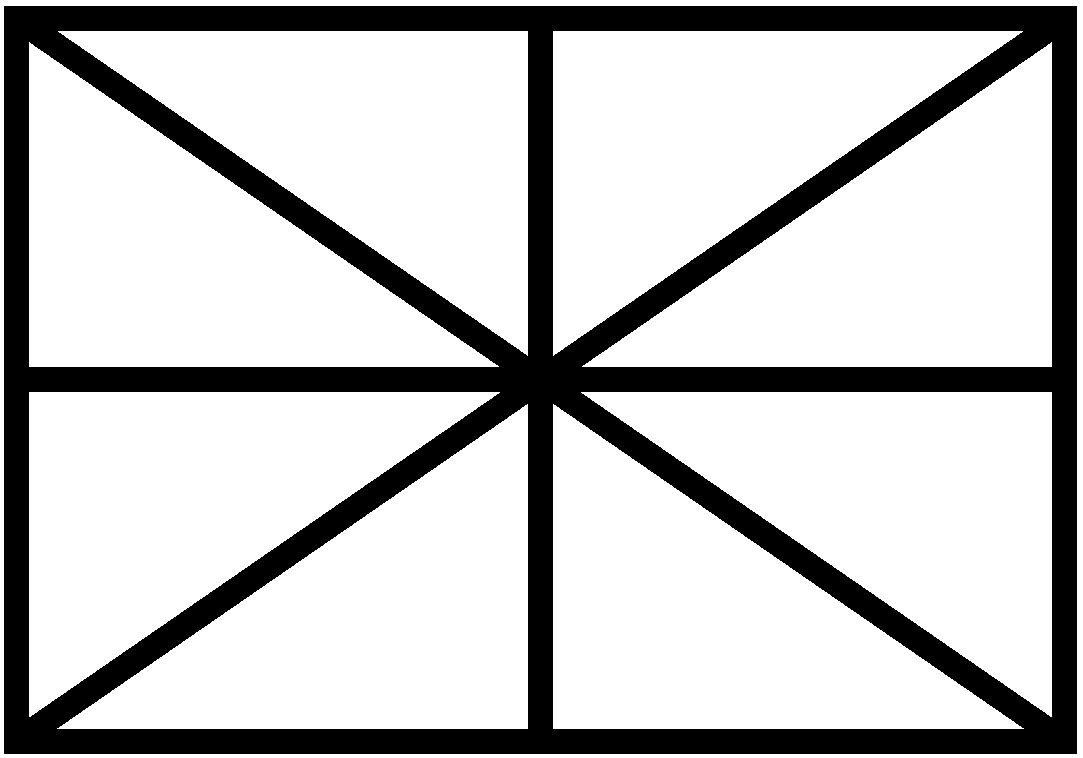
\includegraphics[width=\textwidth]{figure}
% \makeatletter
% \let\@currsize\normalsize
% \caption{Caption.}
% \label{fig:figure}
% \end{figure}
% 
% \begin{figure}[t]
% \centering
% \begin{tabular}{c c}
% \includegraphics[height=2.5in]{figureA} &
% \includegraphics[width=3in]{figureB}\\
% (A) & (B)
% \end{tabular}
% \makeatletter
% \let\@currsize\normalsize
% \caption{Two figures.}
% \label{fig:twofigures}
% \end{figure}

% currsize is not set in the long table environment, so we need to set it before we set it up.
\makeatletter
\let\@currsize\normalsize
\makeatother


\noindent Again, we don't indent here.

\appendix
\addcontentsline{toc}{chapter}{APPENDICES}
\chapter{Third Party Libraries Used}

\noindent Modulo7 is a significant software engineering effort. This is partly due to the fact that Modulo7 tends to address speed related issues that are prevalent in other frameworks and partly due to the disparate sources of music that it supports. As such Modulo7 utilizes a number of third party libraries in its operations. These libraries and their roles are mentioned below:-

\section{Apache Lucene}

\noindent Apache Lucene is a full text search engine library written in Java. Apache Lucene is used for indexing text documents, spelling correction and other such functionality. \\
In context of Modulo7, Apache Lucene is used to maintain inverted indices of lyrics either independently acquired from text files containing lyrics or from emdedded lyrics in the Modulo7 supported sources. 

\section{Apache Avro}

\noindent Apache Avro is a serialization library used to store Modulo7 objects to disk. This allows for faster retrieval of parsed objects instead of having to reparse entire song sources again and again.

\section{Echo Nest jEN API}

\noindent The toughest challenge in all of Modulo7 was to parse symbolic information from audio sources. In order to accomplish this, Modulo7 relied on the Echo Nest's client library to convert mp3 files into chromagram representation of music \cite{chromagramtutorial}. The chromagram representation is acquired directly by converting mp3 representation into the frequency domain by Echo Nest. Modulo7 treats this process as a black box, as it is interested in finding out only the chromagram representation (from which identifying notes and chords become much simpler). 

\section{Antlr}

\noindent Antlr (Another language recognition tool) is a framework used to develop lexers and parses for custom programming languages. In case of Modulo7, Antlr was used to develop the Modulo7SQL Custom query language.

\section{Jsoup}

\noindent Jsoup is a library used for parsing XML documents written in Java. In case of Modulo7, Jsoup is used to parse music xml documents and present song representations to the Modulo7 engine. 

\section{Audiveris}

\noindent Audiveris is a OMR (Optical Music Recognition System) written in Java which converts digitized sheet music files into musicxml files. Audiveris is used to parse sheet music files into Modulo7 song representations.

\section{Alchemy} \label{Alchemy}

\noindent Alchemy is an implementation of NLP(In general AI) as a service model by IBM. Alchemy provides support for language ID, semantic analysis of arbitrary documents and text. In Modulo7, Alchemy is used for analyzing lyrics.  

\section{Apache JCS (Java Caching System)}

\noindent Apache JCS is used as a distributed in memory cache to cache the results of Modulo7 custom queries and similarity results for the queries made in the past. 

\chapter{Algorithms in use in Modulo7}

\noindent There are certain algorithms in literature that are directly implemented in Modulo7. These algorithms facilitate the smooth functioning of Modulo7's indexing in face of incomplete metadata. Some notable algorithms that have been used are briefly described in the following subsections

\section{KK Tonality Profiles and a Key Estimation Algorithm} \label{kktonality}

\noindent Many music sources have the key signature inscribed in it. For example a midi file might have the key signature bytes transcribed. In the event that this information is not present, it must be inferred from the recording. This is required for certain similarity measures that need the key signature of the song for preprocessing steps  in particular for tonality alignment (\ref{sim:unequal}). There are many methods for achieving this including non trivial tree representations of polyphonic music to estimate key \cite{treemodel}. However in Modulo7, the author has implemented a simpler model for tonality estimation based on templates called KK tonality profiles \cite{kkTonalityKeyFinding} \\

\noindent The premise of the KK tonality profile stems from experiments done in \cite{kkTonalityKeyFinding} and \cite{kkcognitive} which estimate how likely a user is to ascribe a note to a series on notes played on a melody or an incomplete harmonic element in different keys. The notes guessed correlate to the relative prominence of a note in a given key(what this the frequency and total duration a note is played in a song in a given key). After many experiments, the experimenters collected the aggregate duration for each note for each key. This experiment was  repeated for all 12 major and 12 minor keys. They were able to acquire 24 profiles (vectors of real numbers) which represent a quantitative measure of the key. For example the profiles for C Major and C Minor are respectively \cite{kkcognitive}.
\begin{equation} \label{kkprofiles}
\begin{aligned}
  CMajor = <6.35, 2.23, 3.48, 2.33, 4.38, 4.09, 2.52, 5.19, 2.39, 3.66, 2.29, 2.88> \\
  CMinor = <6.33, 2.68, 3.52, 5.38, 2.60, 3.53, 2.54, 4.75, 3.98, 2.69, 3.34, 3.17>, 
\end{aligned}
\end{equation}

\noindent The profiles of the other keys can be achieved by rotating the vector by the intervalic distance of the root notes of the key and root note their reference Key(CMajor for major keys and CMinor for minor keys). \\

\noindent The key estimation algorithm leverages the kk tonality profiles as input. The algorithm is as follows:-

\begin{algorithm}

\label{CHalgorithm}
\begin{algorithmic}[1]
\Procedure{Predict Key Signature(song)} {}
\State Define CMaj and CMin as per eqn \ref{kkprofiles}
\State Define MajProf and MinProf = [] % empty sets
\State MajProf.add(CMaj) and MinProf.add(CMin)
\State Define prev\_Key = C 
\For {key in western keys [D to B]}
\State MajProf[key] = left\_shift(MajProf[prev\_Key])
\State MinProf[key] = left\_shift(MinProf[prev\_Key])
\State prev\_Key = key
\EndFor
\State song\_Pitch\_Hist = compute\_song\_tonal\_histogram(song) as per \ref{NPDH}
\State best\_Key = CMin, best\_Corr = $-\infty$
\For {key, maj\_prof in MajProf}:
\If {correlation(maj\_prof, song\_Pitch\_Hist) > best\_Corr}
\State best\_Key = key
\State best\_Corr = correlation(maj\_prof, song\_Pitch\_Hist)
\EndIf
\EndFor
\For {key, mij\_prof in MijProf}:
\If {correlation(min\_prof, song\_Pitch\_Hist) > best\_Corr}
\State best\_Key = key
\State best\_Corr = correlation(min\_prof, song\_Pitch\_Hist)
\EndIf
\EndFor
\Return best\_Key
\EndProcedure
\end{algorithmic}
\end{algorithm}

\subsection{Chord Identification from Chromagram}

\noindent A chromagram \cite{chromagramtutorial} is a representation of a song in frequency domain with relative intensities of notes in a short window frames of analysis in songs. This chromagram representation is central to acquiring symbolic description from audio sources. Once a chromagram is acquired, ascertaining chords in it becomes important(in particular because harmonic elements are non trivial to ascertain in a given chromagram). Modulo7 implements an algorithm described in \cite{chord-detection} in order to detect chords in chromagrams. This procedure is based on chromagram templates of different chords and correlation of current chromagram with these templates.


%% REFERENCES

% if you use BIBTEX
\bibliographystyle{IEEEtran}
\bibliography{thesis}

\end{document}
